%!TeX root=../tese.tex
%("dica" para o editor de texto: este arquivo é parte de um documento maior)
% para saber mais: https://tex.stackexchange.com/q/78101/183146

%% ------------------------------------------------------------------------- %%
\chapter{Árvores splay}
\label{cap:arvores-splay}

\newtheorem{caso}{Caso}

Neste capítulo apresentaremos a estrutura Árvore Splay desenvolvida por \cite{selfadjustingbst}. Descreveremos a implementação e funcionamento das operações splay, access, insert, delete, split e join e analisaremos o custo amortizado da árvore.


\section{Introdução}
O algoritmo tradicional de busca em ABB inicia a execução de um acesso na raiz e desce para o filho apropriado até alcançar a chave procurada. O pior caso é quando a chave procurada está em um nó folha mais profundo. Nesse caso, o algoritmo tem que passar por toda a altura da árvore até chegar a essa folha. Assim, o custo do pior caso é proporcional à altura da árvore que, no pior dos casos é linear $\mathcal{O}(n)$ e no melhor dos casos, tem custo $\mathcal{O}(\log{}n)$.

Com base neste limitante inferior de custo $\Omega(\log{}n)$ para pior caso de buscas em ABBs, foram desenvolvidas uma série de estruturas conhecidas como \textit{árvores binárias de busca balanceadas}. Essas árvores têm o intuito de minimizar a própria altura por meio de rotações e consequentemente mitigar o custo de acessos de pior caso. Muitas dessas estruturas se utilizam de armazenamento de memória adicional por nó para manter informações essenciais para a lógica de balanceamento proposta. 

Apesar dessas estruturas garantirem custo do delimitante inferior $\Theta(\log{}n)$ para o pior caso de busca, elas não conseguem alcançar uma eficiência para um conjunto de buscas superior a essa independente da entrada. Padrões de acesso do mundo real muitas vezes possuem tendências ou estruturas repetitivas, como por exemplo bancos de dados que recebem solicitações frequentes para um pequeno número de elementos de alto tráfego. Em alguns desses casos, é possível ter uma performance melhor que $\mathcal{O}(\log{}n)$ por busca.

Uma alternativa para uma performance melhor é a árvore splay. Árvore Splay é uma árvore binária de busca balanceada proposta por \cite{selfadjustingbst}. Diferentemente das árvores binárias balanceadas citadas anteriormente, a árvore splay se reestrutura após cada operação, inclusive após acessos e não utiliza armazenamento adicional.

A árvore splay é uma ABB que segue a heurística “move to front”, ou seja, a ideia central é que a medida que operações são realizadas na estrutura, os elementos são movidos para perto da raiz de uma maneira particular com intuito de manter na raiz o nó da última chave acessada.
Com a tendência dos nós com chave mais recentemente acessadas estarem próximos da raiz, o custo de sequências de acessos repetitivos tende a diminuir e essas reestruturações também auxiliam a árvore splay a dispor seus nós de maneira mais balanceada, reduzindo a altura total da árvore em alguns casos.

{
    \tikzset{
        nodes = {draw, circle, minimum size = 8mm},
        edge from parent path = {(\tikzparentnode) -- (\tikzchildnode)},
    sibling distance=20pt,
    n/.style = {draw=none},
    r/.style = {fill=white},
    b/.style = {fill=gray},
    edge from parent/.append style={-, shorten >= 0, shorten <= 0}
    }

\section{Operação Splay}

A essência da árvore splay está na operação splay. A operação splay é a responsável por mover um nó específico para a raiz por meio de sucessivas rotações duplas. Essa operação é fundamental para o funcionamento da estrutura e é utilizada por todas as outras operações. 

A operação splay se utiliza de três tipos distintos de rotações para trazer um nó para a raiz: zig, zig-zig e zig-zag.

Seja $x$ o nó que a operação splay está deslocando para a raiz. 

\subsection{Caso zig}

A rotação zig acontece quando $x$ é descendente direto do nó raiz. Neste caso apenas é necessário realizar uma rotação no nó $x$ e $x$ se encontrará na raiz da árvore. Este é o único de rotação única.

Como a operação splay se encerra quando o nó analisado chega a raiz, esta rotação é executada no máximo uma vez durante a execução desta operação. Ela só acontece quando o caminho de $x$ até a raiz da ABB tem comprimento ímpar.

\begin{figure}[h]
    \centering
    \begin{comment}
    \begin{tikzpicture}[
        ed/.style = {densely dashed, shorten >= 5pt},
        alpha/.style = {regular polygon, regular polygon sides=3, draw, minimum size=1.1cm, inner sep=2pt, anchor=south},
        circ/.style = {draw, shape=circle, inner sep=2pt, anchor=south},
        level distance=1.5cm,
        sibling distance=0.5cm
        ]
        
        \begin{scope}[local bounding box=scope1]
        \Tree [.$y$ [.$x$ \node[alpha]{a}; \node[alpha]{b}; ] \node[alpha]{c}; ]
        \end{scope}
        
        \begin{scope}[xshift=6cm, local bounding box=scope2]
        \Tree [.$x$ \node[alpha]{a}; [.$y$ \node[alpha]{b}; \node[alpha]{c}; ] ]
        \end{scope}
        
        \draw[->] ([yshift=-0.5*\ht\strutbox,xshift=0.5cm]scope1.east) -- node [n] {} ([yshift=-0.5*\ht\strutbox,xshift=-0.5cm]scope2.west); % Ajusta a flecha centralizada
        
        \draw[->] ([yshift=-1.65cm, xshift=-0.285cm]scope1.north) arc (180:0:0.7cm);
        
    \end{tikzpicture}
    \end{comment}
    \includegraphics{imagens/zig.pdf}
    \label{fig:zig}

\caption{Caso zig com $x$ nó esquerdo da raiz.}
\end{figure}

\subsection{Caso zig-zig}

A rotação zig-zig é realizada quando $x$ e seu pai possuem a mesma orientação em relação aos seus pais, ou seja, ambos são filhos direitos ou ambos são filhos esquerdos. Neste caso, é necessário rotacionar o pai de $x$ primeiro e em seguida rotacionar $x$.

\begin{figure}[H]
    \centering
    \begin{comment}
    \begin{tikzpicture}[
        ed/.style = {densely dashed, shorten >= 5pt},
        alpha/.style = {regular polygon, regular polygon sides=3, draw, minimum size=1.1cm, inner sep=2pt, anchor=south},
        level distance=1.5cm,
        sibling distance=0.25cm
        ]
        
        \begin{scope}[local bounding box=scope1]
        \Tree [.$z$  [.$y$ [.$x$ \node[alpha]{a}; \node[alpha]{b}; ] \node[alpha]{c};] \node[alpha]{d};]
        \end{scope}
        
        \begin{scope}[xshift=6cm, local bounding box=scope2]
        \Tree [.$x$ \node[alpha]{a}; [.$y$ \node[alpha]{b}; [.$z$ \node[alpha]{c}; \node[alpha]{d}; ]]]
        \end{scope}
        
        \draw[->] ([yshift=-0.5*\ht\strutbox,xshift=0.5cm]scope1.east) -- node [n] {} ([yshift=-0.5*\ht\strutbox,xshift=-0.5cm]scope2.west); % Ajusta a flecha centralizada
        
        \draw[->] ([yshift=-2.20cm, xshift=-0.98cm]scope1.north) arc (198:-18:0.7cm);
        \draw[->,red] ([yshift=-3.67cm, xshift=-1.89cm]scope1.north) arc (198:-18:0.7cm);
    
    \end{tikzpicture}
    \end{comment}
    \includegraphics[scale=0.9]{imagens/zigzig2.pdf}
    \label{fig:zigzig}
\caption{Caso zig-zig com $x$ e $y$ ambos filhos esquerdos.}
\end{figure}


\subsection{Caso zig-zag}

A rotação zig-zag é realizada quando $x$ e seu pai possuem orientação diferentes em relação aos seus pais, ou seja, $x$ é filho direito e o pai de $x$ é filho esquerdo ou $x$ é filho esquerdo e o pai de $x$ é filho direito. Neste caso, é necessário rotacionar $x$ duas vezes. Vale ressaltar que cada rotação será feita para um lado.

Note que esta rotação propositalmente diminui a altura da subárvore analisada.
    
\begin{figure}[H]
    \centering
    \begin{comment}
    \begin{tikzpicture}[
        ed/.style = {densely dashed, shorten >= 5pt},
        alpha/.style = {regular polygon, regular polygon sides=3, draw, minimum size=1.1cm, inner sep=2pt, anchor=south},
        level distance=1.5cm,
        sibling distance=0.25cm
        ]

        \begin{scope}[local bounding box=scope1]
            \Tree [.$z$  [.$y$ \node[alpha]{a}; [.$x$ \node[alpha]{b}; \node[alpha]{c}; ]] \node[alpha]{d};]
        \end{scope}
        
        \begin{scope}[xshift=6cm, local bounding box=scope2]
            \Tree [.$z$  [.$x$ [.$y$ \node[alpha]{a}; \node[alpha]{b}; ] \node[alpha]{c};] \node[alpha]{d};]
            \end{scope}
            
            \begin{scope}[xshift=12cm, local bounding box=scope3]
                \Tree [.$x$ [.$y$ \node[alpha]{a}; \node[alpha]{b};] [.$z$  \node[alpha]{c}; \node[alpha]{d};]]
            \end{scope}
                
            \draw[->] ([yshift=-0.5*\ht\strutbox,xshift=0.3cm]scope2.east) -- node [n] {} ([yshift=-0.5*\ht\strutbox,xshift=-0.3cm]scope3.west);
                
            \draw[->] ([yshift=-3.67cm, xshift=0.67cm]scope2.north) arc (-18:198:0.7cm);
                \draw[->,red] ([yshift=-3.69cm, xshift=-0.82cm]scope2.north) arc (198:-18:0.86cm);
                
    \end{tikzpicture}
    \end{comment}
    \includegraphics[scale=0.85]{imagens/zigzag2.pdf}
    \caption{Caso zig-zag com $x$ filho direito e $y$ filho esquerdo.}
\end{figure}
        
}

Uma série de operações podem ser implementadas nessas estruturas como inserção, remoção, busca, junção e divisão. Todas essas operações chamam a operação splay no nó mais profundo visitado durante sua execução. Para esse trabalho, o importante é saber que a cada acesso, o nó com a chave acessada será levado para a raiz pela operação splay.

\section{Análise da operação splay}

Definimos o custo da operação splay como o número de rotações realizadas durante sua execução. Caso nenhum rotação seja realizada, definimos o custo dessa operação como 1. 

Faremos uma análise amortizada da estrutura. Seja $S$ a árvore splay sendo analisada, $c$ o custo real de uma operação splay e \( \hat{c}\) o custo amortizado de uma operação splay. Definimos $s(x)$ como o tamanho da subárvore enraizada no nó $x$. Definimos o potencial local do nó $x$ como $r(x) = \log_2(s(x))$. Por fim, definimos o potencial da árvore splay inteira como $\Phi$.

\begin{lemma}
    O custo amortizado da execução da operação splay no nó $x$ é $\leq 3(r'(x) - r(x)) + 1$, onde $r$ é o potencial local antes da operação e $r'$ o potencial local depois da operação. $\Phi$ é o potencial da árvore antes da operação e $\Phi'$ o potencial da árvore depois da operação
\end{lemma}

\begin{proof}
    Se o nó $x$ for raiz, o custo da operação é 1 e a limitação é imediata. É necessário analisar os casos zig, zig-zig e zig-zag. Para analisar esses casos, denotemos $y$ como o pai de $x$ antes da operação e $z$ o pai de $y$ antes da operação, se $z$ existir.

    \textit{Caso zig}.   
    \begin{align*}
        \hat{c} &= c + \Delta \Phi,\\
        &= 1 + r'(x) + r'(y) - r(x) - r(y), \quad & \text{}\\
        &\leq 1 + r'(x) - r(x) \quad & \text{pois $r(y) \geq r'(y)$},\\
        &\leq 1 + 3(r'(x) - r(x)) \quad & \text{pois $r'(x) \geq r(x)$}.\\
    \end{align*}

    Para os próximos casos será essencial entender uma propriedade da função logaritmo. A função logaritmo é côncava, ou seja, $\frac{\log_2(a) + \log_2(b)}{2} \leq \log_2(\frac{a+b}{2})$. Isso pode ser evidenciado pela Figura~\ref{fig:log}.

    \begin{figure}
        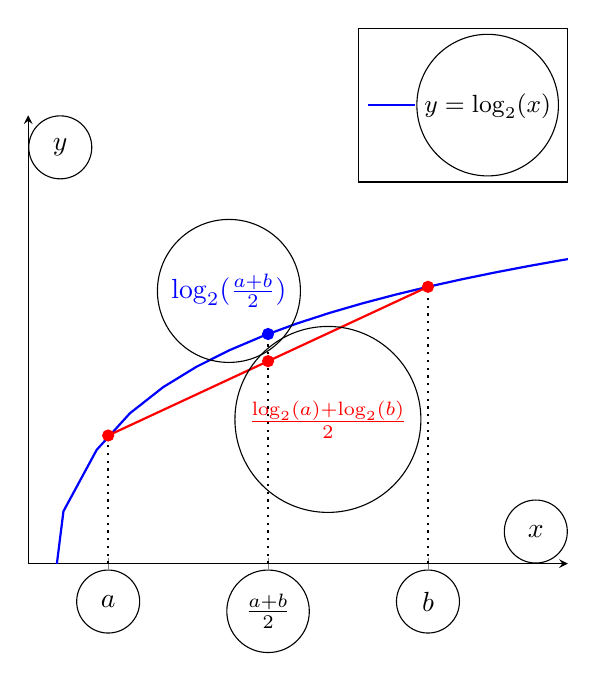
\begin{tikzpicture}
            \begin{axis}[
                axis lines = middle,
                xmin=0, xmax=27,
                ymin=0, ymax=7,
                xtick={4,12,20},
                xticklabels={$a$,$\frac{a+b}{2}$,$b$},
                ytick=\empty,
                xlabel = {$x$}, % Nome do eixo x
                ylabel = {$y$},
                legend style={
                    at={(1,0.85)},  % Move a legenda mais para baixo
                    anchor=south east,
                    font=\small   % Reduz o tamanho da fonte da legenda
                }
            ] % Função y = log2(x)
                \addplot[blue, thick, domain=0.1:40] {log2(x)};
                
                % Pontos
                \addplot[only marks, red] coordinates {(4,2)}; % Ponto A
                \addplot[only marks, red] coordinates {(20, 4.3219281)}; % Ponto B
                \addplot[only marks, blue] coordinates {(12,3.5849625)}; % Ponto C
                \addplot[only marks, red] coordinates {(12,3.16096405)}; % Ponto D
        
                % Reta entre A e B
                \addplot[red, thick] coordinates {(4,2) (20, 4.3219281)};
                
                % Linhas pontilhadas
                \draw[thick, dotted] (axis cs:4,0) -- (axis cs:4,2);   % Linha pontilhada de A
                \draw[thick, dotted] (axis cs:20,0) -- (axis cs:20, 4.3219281);   % Linha pontilhada de B
                \draw[thick, dotted] (axis cs:12,0) -- (axis cs:12, 3.5849625);
                
                % Nomes dos pontos
                \node at (axis cs:12, 3.5849625) [anchor=south east, text = blue, xshift=0.15cm, yshift=-0.1cm] {$\log_2(\frac{a+b}{2})$};  % Nome do ponto C
                \node at (axis cs:12, 3.16096405) [anchor=north west, text=red, xshift=-0.08cm, yshift=0.1cm] {$\frac{\log_2(a) + \log_2(b)}{2}$};  % Nome do ponto D
                
                % Legenda
                \addlegendentry{$y = \log_2(x)$} % Legenda para a função
            \end{axis}
        \end{tikzpicture}
    \caption{Na imagem estão destacados pontos $a$ e $b$ arbitrários na função. Como a função é côncava, o ponto com $y = \frac{\log_2(a) + \log_2(b)}{2}$ nunca estará acima do ponto com $y = \log_2(\frac{a+b}{2})$.}
    \label{fig:log}
    \end{figure}
    
    \textit{Caso zig-zig}.   
    \begin{align*}
        %\hat{c} &= c + \Delta \Phi, & \hspace*{-1.2cm} \text{amortizado = custo + diferença de potencial}, \\
        \hat{c} &= c + \Delta \Phi,\\
        &= 2 + r'(x) + r'(y) + r'(z) - r(x) - r(y) - r(z), \quad & \text{}\\
        &= 2 + r'(y) + r'(z) - r(x) - r(y) \quad & \text{pois $r'(x) = r(z)$},\\
        &\leq 2 + r'(x) + r'(z) - 2r(x) \quad & \text{pois $r(y) \geq r'(y)$}.
    \end{align*}



\end{proof}


\section{Conjectura da Otimalidade Dinâmica}

Uma ABB online é \textit{dinamicamente ótima} se, para todas as sequências $X$, seu algoritmo de busca tem custo O(OPT($X$)). De maneira mais geral, uma ABB online é \textit{$c$-competitiva} se executa todas as sequências $X$ suficientemente longas com custo no máximo $c$\,OPT($X$).

\cite{selfadjustingbst} conjecturaram que a árvore splay é dinamicamente ótima. Essa conjectura é conhecida por Conjectura da Otimalidade Dinâmica. Diversos pesquisadores já investigaram essa conjectura mas ainda pouco se sabe sobre ela. Os resultados obtidos com essas décadas de pesquisa não obtiveram sucesso provando ou refutando essa hipótese, porém provou-se que a árvore splay é uma estrutura que possui muitas propriedades que o custo ótimo também tem.